\section{Assumptions}
During the analysis, we will asume a cache with an LRU eviction policy.
Additionally, we will not take into consideration cache associativity to simplify the analysis.

\section{Spatial Temporal Analysis}
\label{sec:st_analysis}
The memory accesses of an algorithm can be plotted in a spatial-temporal diagram, with the address space on the spatial axis and order of access on the temporal axis.
Since only the thread order can be manipulated, we do not need the granuality of the individual memory accesses within a thread.
This also avoids the problem of threads being concurrent and puts the focus on the temporal locality between threads.
A different thread order shuffles the columns within this diagram: the same data is accessed but simply in a different order.

Additionally, we annotate this diagram with the cache level (L1, L2, RAM) of each memory address by simulating memory.
For the simulation we will use a simple LRU eviction policy which most Nvidia GPUs use and is similar to newer variation on the newer architectures like Turing and Volta, (see section \ref{sec:cache_gpu}).

The resulting spatial temporal diagrams (for example, figure \ref{fig:st_stencil_naive}) have the vertical axis describing the location in a 2D array which is mapped to 1D address space and the horizontal axis describing time. \fsquare{red} are addresses of cache lines that are brought into cache. \fsquare{black} are addresses being accessed. \fsquare{gray} are addresses in cache.

\section{Stencil Operations}

Stencil operation produces an N-dimensional array from a same sized input.
It consists of $I_w \times I_h$ tasks with $I_w$ being the first dimension of the input and $I_h$ being the product over the other dimensions.
For each element it reads a fixed sized $S_w \times S_h$ neighborhood and writes a single element.
Stencils are used for image operations (edge detection, filters, noise reduction), but can also find their use in other fields such as approximating partial differentiation\cite{roth1997compilingstencils} and cellular automata.
For example, a 2-dimensional $5 \times 5$ box blur filter over an input matrix $A$ can be mathemathically defined as:

\begin{equation}
    \texttt{Stencil}(x, y) = %
        \sum_{i=-2}^{2} %
        \sum_{j=-2}^{2} %
        \frac{ A[x + i, y + j] }{25}
    \label{eq:stencil_boxblur}
\end{equation}

In Accelerate, stencils are defined as listing \ref{lst:stencil_signature}, where the stencil function \texttt{stencil -> Exp b} takes in an N-dimensional tuple to produce a single value.
The boundary condition handles how boundary values are handled, either as a predefined function such as \texttt{clamp} and \texttt{mirror}, or as a user defined function.

\begin{listing}[H]
    \begin{minted}{haskell}    
stencil :: forall sh stencil a b. (Stencil sh a stencil, Elt b)	 
    -- stencil function
    => (stencil -> Exp b)
    -- boundary condition
    -> Boundary (Array sh a)	
    -- source array
    -> Acc (Array sh a)	
    -- destination array
    -> Acc (Array sh b)	
    \end{minted}
    \caption{
        The type signature of the stenciling function in Accelerate.
    }
    \label{lst:stencil_signature}
\end{listing}

To implement equation \ref{eq:stencil_boxblur} in Accelerate, we define a function to sum and divide all elements (listing \ref{lst:stencil_usuage}).

\begin{listing}[H]
    \begin{minted}{haskell}
-- Stencil types: included in Data.Array.Accelerate
type Stencil5 a = (Exp a, Exp a, Exp a, Exp a, Exp a) 
type Stencil5x5 a = (Stencil5 a, Stencil5 a, Stencil5 a, Stencil5 a, Stencil5 a) 

-- Example of a 5x5 box blurring stencil filter
boxblur5x5 :: Acc (Matrix Float) -> Acc (Matrix Float)
boxblur5x5 = A.stencil s A.clamp
  where
    -- Take a 5x5 array, then select each element and concatenate them
    s :: Stencil5x5 Float -> Exp Float
    s = average . concatMap (^..each) . (^..each)

    -- average all the elements in a list
    average :: Fractional a => [a] -> a
    average xs = sum xs / genericLength xs
    \end{minted}
    \caption{
        How to use the accelerate stenciling function (listing \ref{lst:stencil_signature}) to produce a $5 \times 5$ box blur filter.
    }
    \label{lst:stencil_usuage}
\end{listing}

\subsection{Naive}
\label{sec:stencil_naive}
The naive implementation iterates over each of the outputs linearly, horizontally first.
The temporal linearity translates to parallelism on GPUs where multiple threads work concurrently on each element of the output array.
The naive implementation of the $5 \times 5$ box blur filter (equation \ref{eq:stencil_boxblur} and listing \ref{lst:stencil_usuage}) is compareable to the following naive CUDA C++ implementation (listing \ref{lst:stencil_cuda}).

\begin{listing}[h]
    \begin{minted}{cuda}
#define STENCIL_SIZE 5

__global__ void stencil_naive(float *output, float *input, int width, int height, int N) {
    int tid = blockIdx.x * blockDim.x + threadIdx.x;
    int x = tid % width;
    int y = tid / width;
    
    if (tid >= N) {
        return;
    }

    float result = 0;
    for (int d_i = -STENCIL_SIZE/2; d_i <= STENCIL_SIZE/2; d_i++) {
        int i = min(height-1, max(0, y + d_i));
        for (int d_j = -STENCIL_SIZE/2; d_j <= STENCIL_SIZE/2; d_j++) {
            int j = min(width-1, max(0, x + d_j));
            result += input[i * width + j];
        }
    }
    output[tid] = result / (STENCIL_SIZE * STENCIL_SIZE);
}
    \end{minted}
    \caption{
        The naive CUDA C++ equivelant to listing \ref{lst:stencil_usuage}
    }
    \label{lst:stencil_cuda}
\end{listing}

While the naive implementation of stencil operations works well enough when enough rows of the input fit in the cache, it begins to fall in performance on larger inputs.
More specifically, inputs that are horizontally wide.

\begin{table}[h]
    \centering
    \begin{tabular}{|c c|}
        \hline
        Cache lines      & 24   \\
        Cache line width & 4    \\
        Eviction policy  & LRU  \\
        \hline
        Stencil size     & 7x7  \\
        Input Size       & 16x16\\
        Column size      & 8    \\
        \hline
    \end{tabular}
    \caption{
        The input parameters to generate the spatial-temporal diagrams for stencil operations.
    }
    \label{tab:sim_stencil_params}
\end{table}

% fig:st_stencil
\begin{figure}[H]
    \centering
    \subfloat[On input sizes too wide (i.e. $16 \times 16$) cache trashing occurs.]{
        \begin{tikzpicture}
            \node (image) at (0,0) {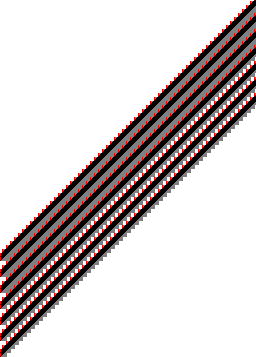
\includegraphics[width=0.4\textwidth]{st_diagrams/stencil7x7_linear.png}};
            \draw [->] (image.south west) -- ++(2,0) node[right]{\footnotesize\textit{Time}};
            \draw [->] (image.south west) -- ++(0,2) node[rotate=90, above]{\footnotesize\textit{Address}};
        \end{tikzpicture}
    }
    \qquad
    \subfloat[The input size is modified to $8 \times 32$ which results in optimal cache utilization.]{
        \begin{tikzpicture}
            \node (image) at (0,0) {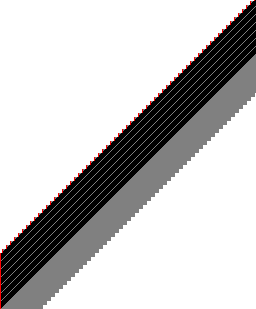
\includegraphics[width=0.4\textwidth]{st_diagrams/stencil7x7_linear_smaller_input.png}};
            \draw [->] (image.south west) -- ++(2,0) node[right]{\footnotesize\textit{Time}};
            \draw [->] (image.south west) -- ++(0,2) node[rotate=90, above]{\footnotesize\textit{Address}};
        \end{tikzpicture}
    }
    \caption{
        The spatial temporal diagram of a 7x7 stencil with linear ordering.
        See section \ref{sec:st_analysis}.
    }
    \label{fig:st_stencil_naive}
\end{figure}

% fig:stencil_naive_loading_pattern
\begin{figure}[!hb]
    \centering
    
    \subfloat[Ideal cache size, only minimal amount of loading is required.]{
        \centering
        \makebox[0.4\columnwidth][c]{
            \begin{tikzpicture}[scale=0.25, decoration = {
                markings, mark = between positions 0.3cm and 0.95 step 0.25cm with {\arrow{stealth}}
            }]
                \fill[gray!50]  ( 6, 6) rectangle +(10, 1);
                \fill[gray!50]  ( 0, 2) rectangle +(16, 4);
                \fill[gray!50]  ( 0, 1) rectangle +(10, 1);
                \fill[gray!100] (10, 1) rectangle +( 1, 1);

                \draw[step=1,gray!25] (0, 0) grid (16, 8);
                \draw[black, postaction = decorate] (8.5, 4.5) -- +(5, 0);
                \draw[black, dashed] (13.5, 4.5) -- (2.5, 3.5);
                \draw[black, postaction = decorate] (2.5, 3.5) -- +(6, 0);
                \draw[red] (6,1) rectangle +(5, 5);
            \end{tikzpicture}
        }
        \label{fig:stencil_naive_loading_pattern_ideal}
    }
    \qquad
    \subfloat[Cache too small, data gets evicted before any potential reuse.]{
        \centering
        \makebox[0.4\columnwidth][c]{
            \begin{tikzpicture}[scale=0.25, decoration = {
                markings, mark = between positions 0.3cm and 0.95 step 0.25cm with {\arrow{stealth}}
            }]
                \fill[gray!50]  (10, 2) rectangle +( 6, 5);
                \fill[gray!50]  ( 0, 1) rectangle +( 8, 5);
                \fill[gray!100] ( 8, 1) rectangle +( 1, 5);

                \draw[step=1,gray!25] (0, 0) grid (16, 8);
                \draw[black, postaction = decorate] (12.5, 4.5) -- +(1, 0);
                \draw[black, dashed] (13.5, 4.5) -- (2.5, 3.5);
                \draw[black, postaction = decorate] (2.5, 3.5) -- +(4, 0);
                \draw[red] (4,1) rectangle +(5, 5);
            \end{tikzpicture}
        }
    }
    \caption{
        Stencil operations require enough cache to prevent chasing.
    }
    \label{fig:stencil_naive_loading_pattern}
\end{figure}

The lower bound of cache in amount of cache lines needed $M_l$ is bounded by the total horizontal footprint $I_w + S_w$ in amount of cache lines $L$, multiplied by the stencil height $S_h$

\begin{equation}
    M_l \geq \ceil{\frac{I_w + S_w}{L}} S_h \label{eq:stencil_naive_optimal_memory}
\end{equation}

While in most cases (such as a $9\times9$ stencil on a $2048\times2048$ array of floating point numbers which takes roughly \~80 KiB of cache.) this enough to fully exploit L2 caches, this can be unoptimal in regard to the L1 cache (64 KiB max on the Turing architecture).
The amount of cache lines needed to be fetched from memory $F$ is bound by the worse case (eq. \ref{eq:stencil_naive_optimal_memory} is not satisfied) where we consistently evict data from cache before we can reuse:

\[
    F \leq \ceil{\frac{I_w + S_w}{L}} I_h S_h
\]

If equation \ref{eq:stencil_naive_optimal_memory} is satisfied, the amount of fetches $F$ is no longer depedent on the stencil height $S_h$

\[
    F = \ceil{\frac{I_w + S_w}{L}} I_h
\]

With multiple threads active, even more data is required to be kept in cache for optimal usuage.
In the best case, all threads are cohesive with overlapping accesses, and in the worst case, threads will be spread out more with less overlapping accesses.
Threads in GPUs are grouped by warps, threads contained within are always cohered, and therefore a guarantee for overlapping accesses.
Therefore, only when multiple warps are executed on the same SM, divergence in accesses can occur.
A single warp of 32 threads uses $\ceil{\frac{32 + S_w}{l}} S_h$ cache lines when the threads cover a single rows. 
When the warp is split between 2 rows, the cache needs to be slightly bigger: $\ceil{\frac{32 + 2 S_w}{l}} S_h$.

Ideally, the whole input array would fit on the cache, but a sufficiently large input (e.g. a $2048\times2048$ 32-bit floating point array uses 16 MiB) will not fit on the L2 caches of modern GPUs ($\approx6$MiB of L2 data cache, Volta V100) and cache misses are unavoidable.
Even if data would fit on the L2 cache, there would still be potential cache misses at the L1 cache (128 KiB, Volta V100).

Using the model by \citeauthor{lam1991cache} and described in section \ref{sec:cache_gpu} can be used to estimate the cache misses of the naive implementation.
However, this requires a simulation to factor in self-interference.

\subsection{Tiling}
\label{sec:stencil_tiled}
A common used optimization is by dividing the work into works as described in \ref{sec:optimization_blocked} and this can be applied to stencil operations as well.

The minimum required cache for optimal tiling is depedent on \TODO{\dots} tiling size $t$

\begin{equation}
    M_l \geq \ceil{\frac{t + S_w}{L}} S_h \label{eq:stencil_tiling_memory}
\end{equation}

The largest possible tiling size $t$ is derived by inverting equation \ref{eq:stencil_tiling_memory}

\begin{equation}
    t \leq \frac{L M_l}{S_h} - S_w
\end{equation}

In practise, equation \ref{eq:stencil_tiling_memory} can be satisfied by adjusting $t$, we can have a lower upper bound on the amount of cache line fetches $F$:

\begin{equation}
    F \leq \ceil{\frac{I_w}{t}} \ceil{\frac{t + S_w}{L}} \ceil{\frac{I_h}{t}} (t + S_h)
    \label{eq:stencil_tiling_fetches}
\end{equation}


\TODO{GPU/multithreading notes}

\section{Matrix Multiplication}

\subsection{Naive}
\label{sec:matrix_naive}
The matrix multiplication of $C = AB$ can be described as $c_{i,j} = \sum_{k}a_{i,k}b_{k,j}$ and can be implemented naively as in listing \ref{lst:mm_naive_cuda}.

\begin{listing}[H]
    \begin{minted}{cuda}
__global__ void matrix_naive(float *o, float *a, float *b, int depth, int width, int height) {
    int tid = blockIdx.x * blockDim.x + threadIdx.x;
    int x = tid % width;
    int y = tid / width;
    
    if (tid >= width * height) {
        return;
    }

    float result = 0;
    for (int i = 0; i < depth; i++) {
        result += a[y * depth + i] * b[x + i * width];
    }
    o[tid] = result;
    
}
    \end{minted}
    \caption{
        The naive CUDA C++ implementation of matrix multiplication
    }
    \label{lst:mm_naive_cuda}
\end{listing}

We run a similar simulation as in section \ref{sec:stencil_naive} with the parameters described in table \ref{tab:sim_matrix_params}.

\begin{table}[H]
    \centering
    \begin{tabular}{|c c|}
        \hline
        Cache lines      & 32   \\
        Cache line width & 4    \\
        Eviction policy  & LRU  \\
        \hline
        Input Size       & 16x16\\
        Column size      & 8    \\
        \hline
    \end{tabular}
    \caption{
        The input parameters to generate the spatial-temporal diagrams for matrix multiplications.
    }
    \label{tab:sim_matrix_params}
\end{table}

% fig:st_matrix
\begin{figure}[H]
    \centering
    \begin{tikzpicture}[spy using outlines={rectangle, magnification=4,connect spies}]
        \node (image) at (0,0) {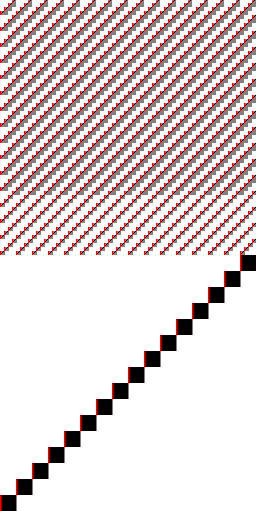
\includegraphics[width=0.25\textwidth]{st_diagrams/matrix_linear.png}};
        \draw [->] (image.south west) -- ++(2,0) node[right]{\footnotesize\textit{Time}};
        \draw [->] (image.south west) -- ++(0,8.5) node[rotate=90, above left]{\footnotesize\textit{Memory Addresses}};

        \coordinate (p) at (0, 1);
        \coordinate (v) at (3.3, 2);
        \spy[width=2.4cm,height=4cm] on (p) in node [fill=white] at (v);
    \end{tikzpicture}

    \caption{
        The spatial temporal diagram of matrix multiplication with linear ordering. 
        See section \ref{sec:st_analysis}.
    }
    \label{fig:st_matrix_naive}
\end{figure}

Given the output matrix $C$ of size $I_w \times I_h$ with input matrices $A$ and $B$ of size $I_w \times D$ and $D \times I_h$ respectively, data from $B$ can be reused in the naive case only if we can both keep one row of $B$ and one column of $A$ loaded.

\begin{equation}
    \label{eq:mm_naive_minimum_cache}
    M_l > \ceil{\frac{D}{L}} + D
\end{equation}

\noindent
If equation \ref{eq:mm_naive_minimum_cache} is satisfied, the amount of cacheloads is roughly

\begin{equation}
    F \approx \ceil{\frac{D}{L}} I_h + D I_w I_h
\end{equation}

\noindent
In the case that equation \ref{eq:mm_naive_minimum_cache} is not satisfied, there is no reuse of data possible, and the amount of cache line fetches is

\begin{equation}
    F \approx \left( \ceil{\frac{D}{L}} + D \right) I_w I_h
\end{equation}

\noindent
To reuse date from both matrix $A$ and $B$ requires to keep the entirity of $A$ cached until we work on the second row.

\begin{equation}
    M_l > \ceil{\frac{D}{L}} + \ceil{\frac{I_w D}{L}}
\end{equation}

\noindent
This lowers the amount of cache loads significantly

\begin{equation}
    F \approx \ceil{\frac{D}{L}} I_h + \ceil{\frac{I_w}{L}} D
\end{equation}

\subsection{Tiling}
Tiling is a common optimization technique for matrix multiplication.
\citet{lam1991cache} suggests a tiling size (\citeauthor{lam1991cache} use the term blocking factor) of $\sqrt{C/2}$ since at that point self interference is minimum.

(Single) Precision General Matrix Multiplication (SGEMM) in Nvidia's implementation of Basic Linear Algebra Subroutines (BLAS) named cuBLAS is a closed sourced library that implements a very optimized GPU based matrix multiplication.
We can, however, look into implementation of GEMM in CUTLASS, an open source alternative to cuBLAS which performs within 80-100\% of cuBLAS depending on platform and workload.
CUTLASS uses a hierarchial structure for tiling putting the outer product first and foremost.